\section{Results}

\begin{figure}[H]
    \centering
    \begin{subfigure}{0.55\textwidth}
        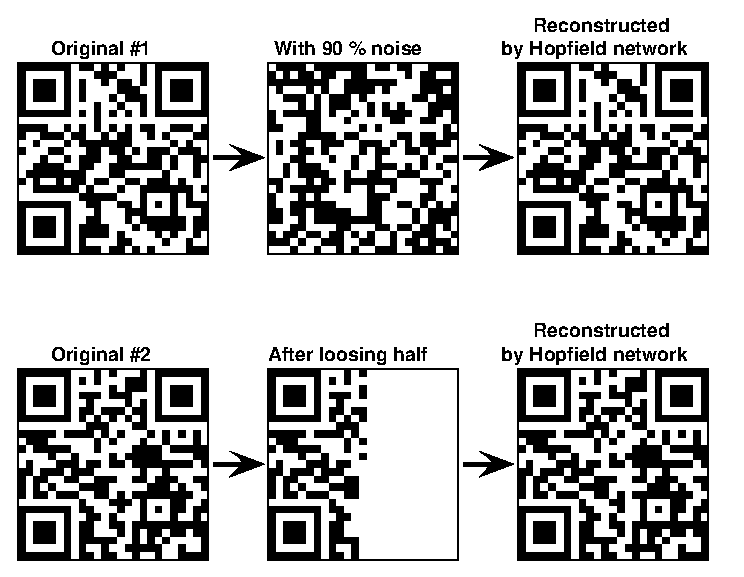
\includegraphics[width=\textwidth]{figs/qr-code}
        \caption{The QR-code contains information encoded within the patterns. A QR decoding app, either online or on a smartphone, can be used to decode the "hidden" message.}
    \end{subfigure}
    \begin{subfigure}{0.4\textwidth}
        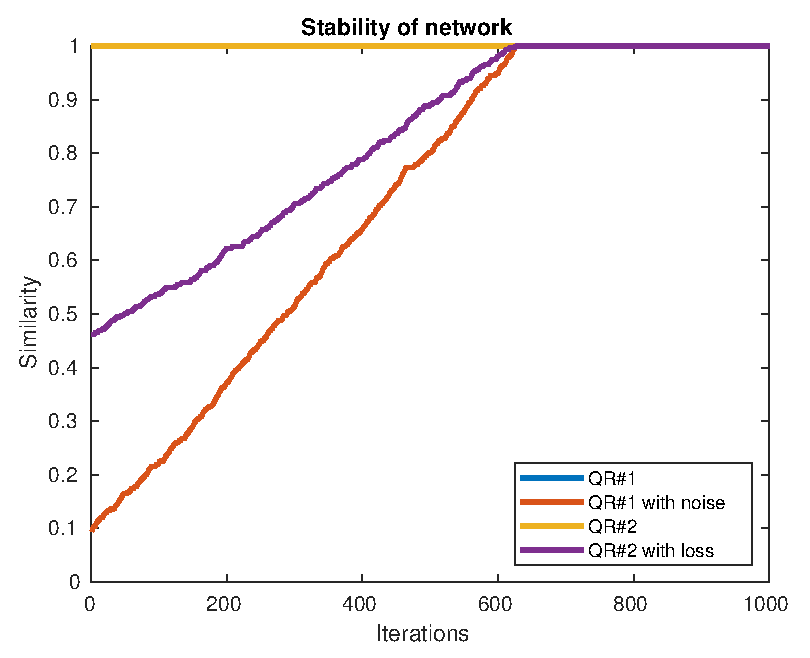
\includegraphics[width=\textwidth]{figs/qr-code-sim}
        \caption{The similarity between the current state of the network and the original QR-code.}
    \end{subfigure}
    \caption{By applying the Hopfield network to a very noisy QR-code we are able to reconstruct the original. By using any QR-code reader we are able to decode the first and last QR-code, while the middle one contains too much noise.}
\end{figure}